\documentclass[]{article}

\usepackage[utf8]{inputenc}
\usepackage[english]{babel}
\usepackage{amsthm}
\usepackage{amssymb}
\usepackage{amsmath}
\usepackage{minted}
\usepackage{tikz}
\newtheorem{theorem}{Theorem}[section]
\newtheorem{lemma}[theorem]{Lemma}
\theoremstyle{definition}
\newtheorem{claim}[theorem]{Claim}


\begin{document}
\section{WFI or not?}
\begin{minted}{haskell}
take 0 xs     = []
take n []     = []
take n (x:xs) = [x]++(take (n-1) xs)
\end{minted}
\begin{minted}{haskell}
drop 0 xs     = xs
drop n []     = []
drop n (x:xs) = drop (n-1) xs
\end{minted}
\begin{claim}The following equation holds.
\begin{minted}{haskell}
(take n xs)++(drop n xs) = xs
\end{minted}
\end{claim}
\begin{proof} by induction over n.
\begin{itemize}
\item[BC:]n=0:
\begin{minted}{haskell}
  (take n xs)++(drop n xs) 
= (take 0 xs)++(drop 0 xs)
= []++xs
= xs
\end{minted}
\item[IH:]
\begin{minted}{haskell}
(take n' xs)++(drop n' xs) = xs
\end{minted}
holds for an arbitrary but fixed n' and all xs.
\item[IS:]n=n'+1
\subitem Case 1: xs=[]
\begin{minted}{haskell}
	  (take n xs)++(drop n xs)
	= (take (n'+1) [])++(drop (n'+1) []) 
	= []++[]
	= []
	= xs
\end{minted}
\subitem Case 2: xs=(x:xs')
\begin{minted}{haskell}
	  (take n xs)++(drop n xs)
	= (take (n'+1) (x:xs'))++(drop (n'+1) (x:xs'))
	= [x]++(take n' xs')++(drop n' xs')
	= [x]++xs'
	= xs
\end{minted}
\end{itemize}
\end{proof}
\newpage
\begin{minted}{haskell}
zip [] ys         = []
zip xs []         = []
zip (x:xs) (y:ys) = [(x,y)]++(zip xs ys)
\end{minted}
\begin{minted}{haskell}
length []     = 0
length (x:xs) = 1+(length xs)
\end{minted}
\begin{minted}{haskell}
min x y
   |x>y   = y
   |true  = x
\end{minted}
\begin{claim}\label{minZip}The following equation holds.
\begin{minted}{haskell}
length (zip xs ys) = min (length xs) (length ys)
\end{minted}
\end{claim}

\begin{proof} by structural induction over xs.
\begin{itemize}
\item[BC:]xs=[]
\begin{minted}{haskell}
  length (zip xs ys)
= length (zip [] ys)
= length []
= 0
= min 0 (length ys) --since (length ys) >= 0
= min (length xs) (length ys)
\end{minted}
\item[IH:]
\begin{minted}{haskell}
length (zip xs' ys) = min (length xs') (length ys)
\end{minted}
holds for an arbitrary but fixed xs' and all ys.
\item[IS:]xs=(x:xs')
\subitem Case 1: ys=[]
\begin{minted}{haskell}
	  length (zip xs ys)
	= length (zip (x:xs') []) 
	= length []
	= min (length (x:xs')) 0 --since (length (x:xs')) > 0
	= min (length xs) (length ys)
\end{minted}
\subitem Case 2: ys=(y:ys')
\begin{minted}{haskell}
	  length (zip xs ys)
	= length (zip (x:xs') (y:ys')) 
	= length ([(x,y)]++(zip xs' ys'))
	= 1+length (zip xs' ys')
	= 1+(min (length xs') (length ys'))
	= min (1+(length xs')) (1+(length ys'))
	= min (length (x:xs')) (length (y:ys'))
	= min (length xs) (length ys)
\end{minted}
\end{itemize}
\end{proof}
But now just for the fun of it let us proof Claim \ref{minZip} by well founded induction.
\begin{align*}
%([],ys)&\prec((x:xs),\hphantom{(y:\ }ys\hphantom{)})\\
%(xs,[])&\prec(\hphantom{(x:\ }xs\hphantom{)},(y:ys))\\
(xs,ys)&\prec((x:xs),(y:ys))
\end{align*}
We denote the transitive closure of $\prec$ by $<$. Obviously $<$ is a well-founded order.
\begin{proof} by well-founded induction with the predicate 
\begin{minted}{haskell}
P((xs,ys))=(length (zip xs ys) = min (length xs) (length ys))
\end{minted}.
%\iff intestead of = ?
\begin{itemize}
\item[] xs=[]: (Note that ([],ys) has no successors w.r.t. $<$.)
\begin{minted}{haskell}
  length (zip xs ys)
= length (zip [] ys)
= length []
= 0
= min 0 (length ys) --since (length ys) >= 0
= min (length xs) (length ys)
\end{minted}
\item[] ys=[]: This case can be treated analogously to xs=[].
\item[] xs=(x:xs'),ys=(y:ys)
\begin{minted}{haskell}
  length (zip xs ys)
= length (zip (x:xs') (y:ys')) 
= length ([(x,y)]++(zip xs' ys'))
= 1+(length (zip xs' ys'))
= 1+(min (length xs') (length ys')) {-since (xs',ys')<(xs,ys) 
                                         P((xs',ys')) holds-}
= min (1+(length xs')) (1+(length ys'))
= min (length (x:xs')) (length (y:ys'))
= min (length xs) (length ys)
\end{minted}
\end{itemize}
\end{proof}
\newpage
\subsection{Lexicographic Order}
\begin{minted}{haskell}
a 0 m = m+1
a n 0 = a (n-1) 1
a n m = a (n-1) (a n (m-1))
\end{minted}
\begin{minted}{haskell}
alist []     ys     = [1]++ys
alist (x:xs) []     = alist xs [x]
alist (x:xs) (y:ys) = alist xs (alist (x:xs) ys)
\end{minted}
\begin{claim}The following equation holds.
\begin{minted}{haskell}
length (alist xs ys) = a (length xs) (length ys)
\end{minted}
\end{claim}
\begin{align*}
(xs,ys)&\prec_l(\hphantom{(x:\ }xs\hphantom{)},(y:ys))\\
(xs,zs)&\prec_l((x:xs),\hphantom{(x:\ }ys\hphantom{)})
\end{align*}
We denote the transitive closure of $\prec_l$ by $<_l$. Obviously $<_l$ is a well-founded order.
\begin{proof} by well-founded induction with the predicate 
\begin{minted}{haskell}
P((xs,ys))=(length (alist xs ys) = a (length xs) (length ys))
\end{minted}
\begin{itemize}
\item[] xs=ys=[]: (Note that ([],[]) has no successors w.r.t. $<_l$.)
\begin{minted}{haskell}
  length (alist xs ys)
= length (alist [] [])
= length ([1]++[])
= 1
= a 0 0
= a (length []) (length [])
\end{minted}
\item[] xs=(x:xs')
\subitem Case 1: ys=[]
\begin{minted}{haskell}
	  length (alist xs ys)
	= length (alist (x:xs') []) 
	= length (alist xs' [x])
	= a (length xs') (length [x]) 
              {-since (xs',[x])<_l(xs,ys) 
                      P((xs',[])) holds-}
	= a (length xs') 1
	= a ((length xs')+1) 0
	= a (length (x:xs')) (length [])
	= a (length xs) (length ys)
\end{minted}
\subitem Case 2: ys=(y:ys)
\begin{minted}{haskell}
	  length (alist xs ys)
	= length (alist (x:xs') (y:ys')) 
	= length (alist xs' (alist (x:xs') ys'))
	= a (length xs') (length (alist (x:xs') ys')) 
	                {-since (xs',(alist (x:xs') ys'))<_l(xs,ys) 
	                       P((xs',(alist (x:xs') ys'))) holds-}
	= a (length xs') (a (length (x:xs')) (length ys'))
	                {-since (xs,ys')<_l(xs,ys) 
	                        P((xs,ys') holds-}
	= a (length xs') (a ((length xs')+1) (length ys'))
	= a ((length xs')+1) ((length ys')+1)
	= a (length (x:xs')) (length (y:ys'))
	= a (length xs) (length ys)
\end{minted}
\end{itemize}
\end{proof}
\subsection{Multiset Order}
\begin{minted}{haskell}
r []     = []
r (0:xs) = r xs
r (x:xs) = r (xs++[(x-1)]++[(x-1)])
\end{minted}
\begin{claim}The following equation holds.
\begin{minted}{haskell}
r xs = []
\end{minted}
\end{claim}
%multiset order

\newpage
%infinitely branching :(
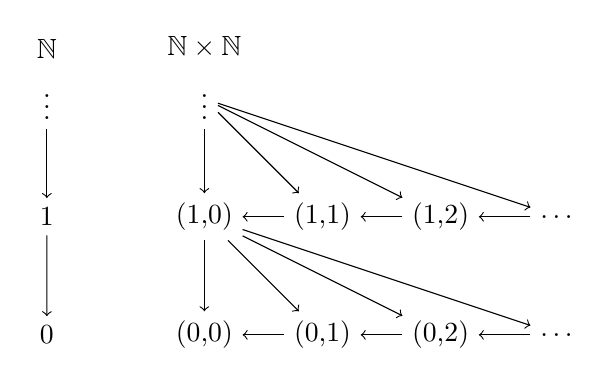
\begin{tikzpicture}[node distance=1.5cm,->,level/.style={level distance = 1.5cm},tree/.style = {align=right}] 
\node [label=above:$\mathbb{N}$] at (0,0) {$\vdots$} 
	child{ node {1}
		child{ node {0}
		}
	};
\node [label=above:$\mathbb{N\times N}$] (a) at (2,0) {$\vdots$}
	child{ node (b1) [below of = a] {(1,0)}
		child{ node (c1) [below of = b1] {(0,0)}	}
		child{ node (c2) [right of = c1] {(0,1)}	}
		child{ node (c3) [right of = c2] {(0,2)}	}
		child{ node (c4) [right of = c3] {$\dots$}	}
	}
	child{ node (b2) [right of = b1] {(1,1)}	}
	child{ node (b3) [right of = b2] {(1,2)}	}
	child{ node (b4) [right of = b3] {$\dots$}	}
	;
	\draw (b2) to (b1);
	\draw (b3) to (b2);
	\draw (b4) to (b3);
	\draw (c2) to (c1);
	\draw (c3) to (c2);
	\draw (c4) to (c3);
\end{tikzpicture}\\
$\mathbb{N}\rightarrow$ finitely branching.\\
$\mathbb{N\times N}\rightarrow$ infinitely branching.\\
Assume there exits a bijective mapping $B:\mathbb{N\times N}\to\mathbb{N}$ such that 
\begin{align*}
(a,b)<_{lex}(c,d) \textbf{ iff } B((a,b))<B((c,d))
\end{align*}holds.
Let $B((1,0))=k$ and consider the increasing chain $(0,0)<_{lex}\dots<_{lex}(0,k)<_{lex}(1,0)$. This chain has $k+2$ elements, the pigeon principle implies 
\end{document}
